\section{Graph Programs}
\label{sec:programs}

We discuss a number of example programs to familiarize the reader with the features of GP and their use in solving graph problems. At the end of the section, we define the abstract syntax of GP programs. 

\begin{example}[Transitive closure]
\label{ex:trans_closure}

A \emph{transitive closure} of a graph is obtained by inserting an edge between all distinct nodes $v$ and $w$ such that there is a directed path from $v$ to $w$ but no edge. The program \texttt{trans\_closure} in Figure \ref{fig:trans_closure} generates a transitive closure of an integer-labelled input graph by applying the rule schema \texttt{link} as long as possible, using the iteration operator '\texttt{!}'. In general, arbitrary command sequences can be iterated. 

\begin{figure}[htb]
 \begin{center}
  \input{Programs/trans_closure.prog}
 \end{center}
\caption{The program \texttt{trans\_closure}\label{fig:trans_closure}}
\end{figure}

The keyword \texttt{main} starts the main command sequence of a program to distinguish it from macros (see Example \ref{ex:2-colouring}). Note that the condition $\mathtt{not\: edge(1,3)}$ of \texttt{link} prevents the creation of edges between nodes that are already linked. Without this condition, \texttt{trans\_closure} could generate parallel edges between nodes 1 and 3 ad infinitum. 

By our definition of transitive closure, we can choose any label for the edge created by \texttt{link}. Using $\mathtt{a+b}$ implies that \texttt{trans\_closure} may produce different results for a given input graph if there are different paths between two nodes. If we want to generate a unique transitive closure, we can replace $\mathtt{a+b}$ with a constant such as $\mathtt{0}$.
\end{example}

\begin{example}[Inverse]
\label{ex:inverse}

The \emph{inverse} of a graph is obtained by reversing the directions of all edges. The  program \texttt{inverse} in Figure \ref{fig:inverse} computes the inverse of an integer-labelled input graph in two stages, using the sequential composition of the loops  \texttt{reverse!} and \texttt{unmark!}. The first loop reverses each edge and replaces its label $x$ with the \emph{tagged}\/ label $x\_\mathtt{0}$, then the second loop removes all tags. In general, arbitrary subprograms can be joined by the semicolon operator. 

\begin{figure}[htb]
 \begin{center}
  \input{Programs/inverse.prog}
 \end{center}
\caption{The program \texttt{inverse}\label{fig:inverse}}
\end{figure}

The underscore operator allows to add a \emph{tag} to a label, used here to mark an edge as having been reversed. In general, a tagged label is a sequence of expressions joined by underscores. Here, we need to mark reversed edges as otherwise the loop \texttt{reverse!} would not terminate. Note that the rule schema \texttt{reverse} can only be applied to edges with untagged labels. 
\end{example}

\begin{example}[Shortest distances]
\label{ex:distances}
Given a graph $G$ whose edge labels are integers, the \emph{distance} of a directed path from a node $v$ to a node $w$ is the sum of the edge labels on that path. If all edge labels in $G$ are nonnegative, then the \emph{shortest distance} from $v$ to $w$ is the minimum of the distances of all paths from $v$ to $w$. 

The program \texttt{distances} in Figure \ref{fig:distances} expects an integer-labelled input graph where exactly one node $v$ has a tagged label of the form $x\_\mathtt{0}$ and where all edge labels are nonnegative. It adds to each node $w$ that is distinct and reachable from $v$ a tag with the shortest distance from $v$ to $w$. 

\begin{figure}[htb]
 \begin{center}
  \input{Programs/distances.prog}
 \end{center}
\caption{The program \texttt{distances}\label{fig:distances}}
\end{figure}
\end{example}

In each iteration of the program's loop, one of the rule schemata \texttt{add} and \texttt{reduce} is applied to the current graph. If both rule schemata are applicable, one of them is chosen nondeterministically. An equivalent, slightly more deterministic solution is to separate the phases of addition and reduction: $\mathtt{main} = \mathtt{add!;\, reduce!}$. A refined version of the program \texttt{distances} which implements Dijkstra's shortest-path algorithm can be found in \cite{Plump-Steinert04a}.

\begin{example}[Colouring]
\label{ex:colouring}
A \emph{colouring} for a graph is an assignment of colours (integers) to nodes such that the source and target of each edge have different colours. The program \texttt{colouring} in Figure \ref{fig:colouring} produces a colouring for every integer-labelled input graph without loops, recording colours as tags. (Checking for loops would be a straightforward extension which we omit for simplicity.) 

\begin{figure}[htbp]
\label{fig:colouring}
 \begin{center}
  \begin{tikzpicture} [scale=0.75,align=center,auto,inner sep=2mm,arrowin,arrowout,font=\ttfamily]

\tikzstyle{every text node part}=[font=\small]

\node at (1.55,2.1) {Main = init!; inc!};
\node at (0.8,1.3) {init(x: list)};
\node at (0,0)[circle,draw,inner sep=2.5mm,label=below:\scriptsize{1}]{x};
\node at (1.5,0){$\Rightarrow$};
\node at (3,0)[circle,draw,inner sep=1.5mm,fill=black!20,label=below:\scriptsize{2}]{x:1};

\begin{scope}[inner sep=1.5mm,xshift=6cm]
\node at (1.7,1.3) {inc(a,x,y:list; i:int)};

\node (l1) at (0,0)[circle,draw,fill=black!20,label=below:\scriptsize{1}]{x:i};
\node (l2) at (2.5,0)[circle,draw,fill=black!20,label=below:\scriptsize{2}]{y:i}
  edge [<-] node[above]{a} (l1);

\node at (4,0){$\Rightarrow$};

\node (r1) at (5.5,0)[circle,draw,fill=black!20,label=below:\scriptsize{1}]{x:i};
\node (r2) at (8,0)[circle,draw,inner sep=0.2mm,fill=black!20,label=below:\scriptsize{2}]{y:i+1}
  edge [<-] node[above]{a} (r1);
\end{scope}

\end{tikzpicture}

  \vspace*{1.5cm}
  \input{Graphs/colour_results.graph}
 \end{center}
\caption{The program \texttt{colouring} and two of its derivations}
\end{figure}

The program initially colours each node with zero and then repeatedly increments either the source or the target colour of an edge with the same colour at both ends. Note that this process is highly nondeterministic: Figure \ref{fig:colouring} shows two different colourings produced for the same input graph, where one is optimal in that it uses only two colours while the other uses four colours. (The problem to generate a colouring with a minimal number of colours is NP-complete \cite{Garey-Johnson79a} and requires a more involved program.)

It is easy to see that whenever \texttt{colouring} terminates, the resulting graph is a correctly coloured version of the input graph. For, the output cannot contain an edge with the same colour at both nodes as then \texttt{inc1} or \texttt{inc2} would have been applied at least one more time. It is less obvious though that the program does terminate for every input graph. 

To see that \texttt{colouring} always terminates, consider graphs  whose node labels are of the form $n\_i$, with $n,i \in \Z$. Given a node $v$, we  denote the tag of its label by $\tag(v)$. Now observe that if $G$ is a graph with $\tag(v) =0 $ for each node $v$, then for every derivation $G \der_{\{\mathtt{inc1},\mathtt{inc2}\}} H$\/ there is some $0 \leq k < V_H$ such that $\tag(V_H) = \{0,1,\dots,k\}$ (where some tags may occur repeatedly in $H$). Thus, by assigning to every graph $M$\/ the integer $\#M = \sum_{v \in V_M} \tag(v)$, we obtain
 \[ \#H < 1+2+ \dots + |V_H| = 1+2+ \dots + |V_G|. \]  
Since $\#H$ equals the number of rule schema applications in $G \der H$, it follows that every derivation with \texttt{inc1} and \texttt{inc2} starting from $G$ must eventually terminate. Moreover, as the upper bound for $\#H$ is quadratic in $|V_G|$, \texttt{colouring} always performs at most a quadratic number of rule schema applications.
\end{example}

\begin{example}[2-Colouring]
\label{ex:2-colouring}
A graph is \emph{2-colourable} (or \emph{bipartite}) if it possesses a colouring with at most two colours. The program \texttt{2-colouring} in Figure \ref{fig:2colouring} generates a 2-colouring for a nonempty and connected input graph if such a colouring exists---otherwise the input graph is returned. The program uses the \emph{macro} \texttt{colour} to represent the rule-schema set $\mathtt{\{colour1,\, colour2\}}$. 

\begin{figure}[htb]
 \begin{center}
  \input{Programs/2colouring.prog}
 \end{center}
\caption{The program \texttt{2-colouring}}\label{fig:2colouring}
\end{figure}

Given an integer-labelled input graph, first the rule schema \texttt{choose} colours an arbitrary node by replacing its label $x$ with $x\_0$. Then the loop \texttt{colour!} applies the rule schemata \texttt{colour1} and \texttt{colour2} as long as possible to colour all remaining nodes. In each iteration of the loop, an uncoloured node adjacent to an already coloured node $v$ gets the colour in $\{0,1\}$ that is complementary to $v$'s colour. If the input graph is connected, the graph resulting from \texttt{colour!} is correctly coloured if and only if the rule schema \texttt{illegal} is not applicable.  The latter is checked by the if-statement. If \texttt{illegal} is applicable, then the input must contain an undirected cycle of odd length and hence is not 2-colourable (see for example \cite{Kleinberg-Tardos06a}). In this case the loop \texttt{undo!} removes all tags to return the input graph unmodified. Note that the number of rule-schema applications performed by \texttt{2-colouring} is linear in the number of input nodes.

We can extend \texttt{2-colouring}'s applicability to graphs that are possibly empty or disconnected by inserting a nested loop: 
\[ \text{\texttt{main = (choose; colour!)!; if illegal then undo!}.} \]
Now if the input graph is empty, \texttt{choose} fails which causes the outer loop to terminate and return the current (empty) graph. On the other hand, if the input consists of several connected components, the body of the outer loop is repeatedly called to colour each component. 
\end{example}

\begin{example}[Series-parallel graphs]
\label{ex:series-parallel}

The class of \emph{series-parallel}\/ graphs is inductively defined as follows. Every graph $G$ consisting of two nodes connected by an edge is series-parallel, where the edge's source and target are called \emph{source} and \emph{target}\/ of $G$. Given series-parallel graphs $G$ and $H$, the graphs obtained from the disjoint union $G + H$\/ by the following two operations are also series-parallel. \emph{Serial composition:}\/ merge the target of $G$ with the source of $H$; the source of $G$ becomes the new source and the target of $H$\/ becomes the new target. \emph{Parallel composition:}\/ merge the source of $G$ with the source of $H$, and the target of $G$ with the target of $H$; sources and targets are preserved.

It is known \cite{Bang_Jensen-Gutin00a,Duffin65a} that a graph is series-parallel if and only if it reduces to a graph consisting of two nodes connected by an edge by repeated application of the following operations: (a) Given a node with one incoming edge $i$ and one outgoing edge $o$ such that $s(i) \neq t(o)$, replace $i$, $o$ and the node by an edge from $s(i)$ to $t(o)$. (b) Replace a pair of parallel edges by an edge from their source to their target. 

Suppose that we want to check whether a connected, integer-labelled graph $G$ is series-parallel and, depending on the result, execute either a program $P$\/ or a program $Q$ on $G$. We can do this with the program
\[ \begin{array}{l}
    \text{\texttt{main = if reduce!; base then $P$\/ else $Q$}}\\
    \mathtt{reduce} = \{\mathtt{serial,\, parallel}\}
   \end{array} \]
whose rule schemata \texttt{serial}, \texttt{parallel} and \texttt{base} are shown in Figure \ref{fig:series-parallel}. 

\begin{figure}[htb]
 \begin{center}
  \input{Programs/series-parallel.prog}
 \end{center}
\caption{Rule schemata for recognizing series-parallel graphs}
\label{fig:series-parallel}
\end{figure}

The subprogram \texttt{reduce!} applies as long as possible the operations (a) and (b) to the input graph $G$, then the rule schema \texttt{base} checks if the resulting graph consists of two nodes connected by an edge. Graph $G$ is series-parallel if and only if \texttt{base} is applicable to the reduced graph. (Note that \texttt{reduce!} preserves connectedness and that, by the dangling condition, \texttt{base} is applicable only if the images of its left-hand nodes have degree one.) If \texttt{base} is applicable, then program $P$\/ is executed, otherwise program $Q$. It is important to note that $P$\/ or $Q$ is executed \emph{on the input graph $G$}\/ whereas the graph resulting from the test is discarded. The precise semantics of the branching command is given in the next section.

To make the above program usable for possibly disconnected graphs, we can add an if-statement which checks whether the application of \texttt{base} has resulted in a nonempty graph: 
\[ \text{\texttt{main = if (reduce!; base; if nonempty then fail) then $P$\/ else $Q$.}} \]
Here \texttt{nonempty} is a rule schema whose left-hand side is a single interface node, labelled with an integer variable. If \texttt{nonempty} is applicable, then the graph resulting from \texttt{reduce!} is disconnected and hence the input graph is not series-parallel. In this case \texttt{fail} causes the test of the outer if-statement to fail, with the consequence that program $Q$ is executed on the input graph.
\end{example}

\begin{example}[Sierpinski triangles]
\label{ex:sierpinski}
A \emph{Sierpinski triangle} is a self-similar geometric structure which can be recursively defined \cite{Peitgen-Juergens-Saupe04a}. Figure \ref{fig:sierpinski} shows a Sierpinski triangle of generation three, composed of three second-generation triangles, each of which consists of three triangles of generation one. The triangle and its geometric layout have been generated with the GP programming system \cite{Taentzer_et_al08a,Manning-Plump08b}.

\begin{figure}[htb]
 \begin{center}
  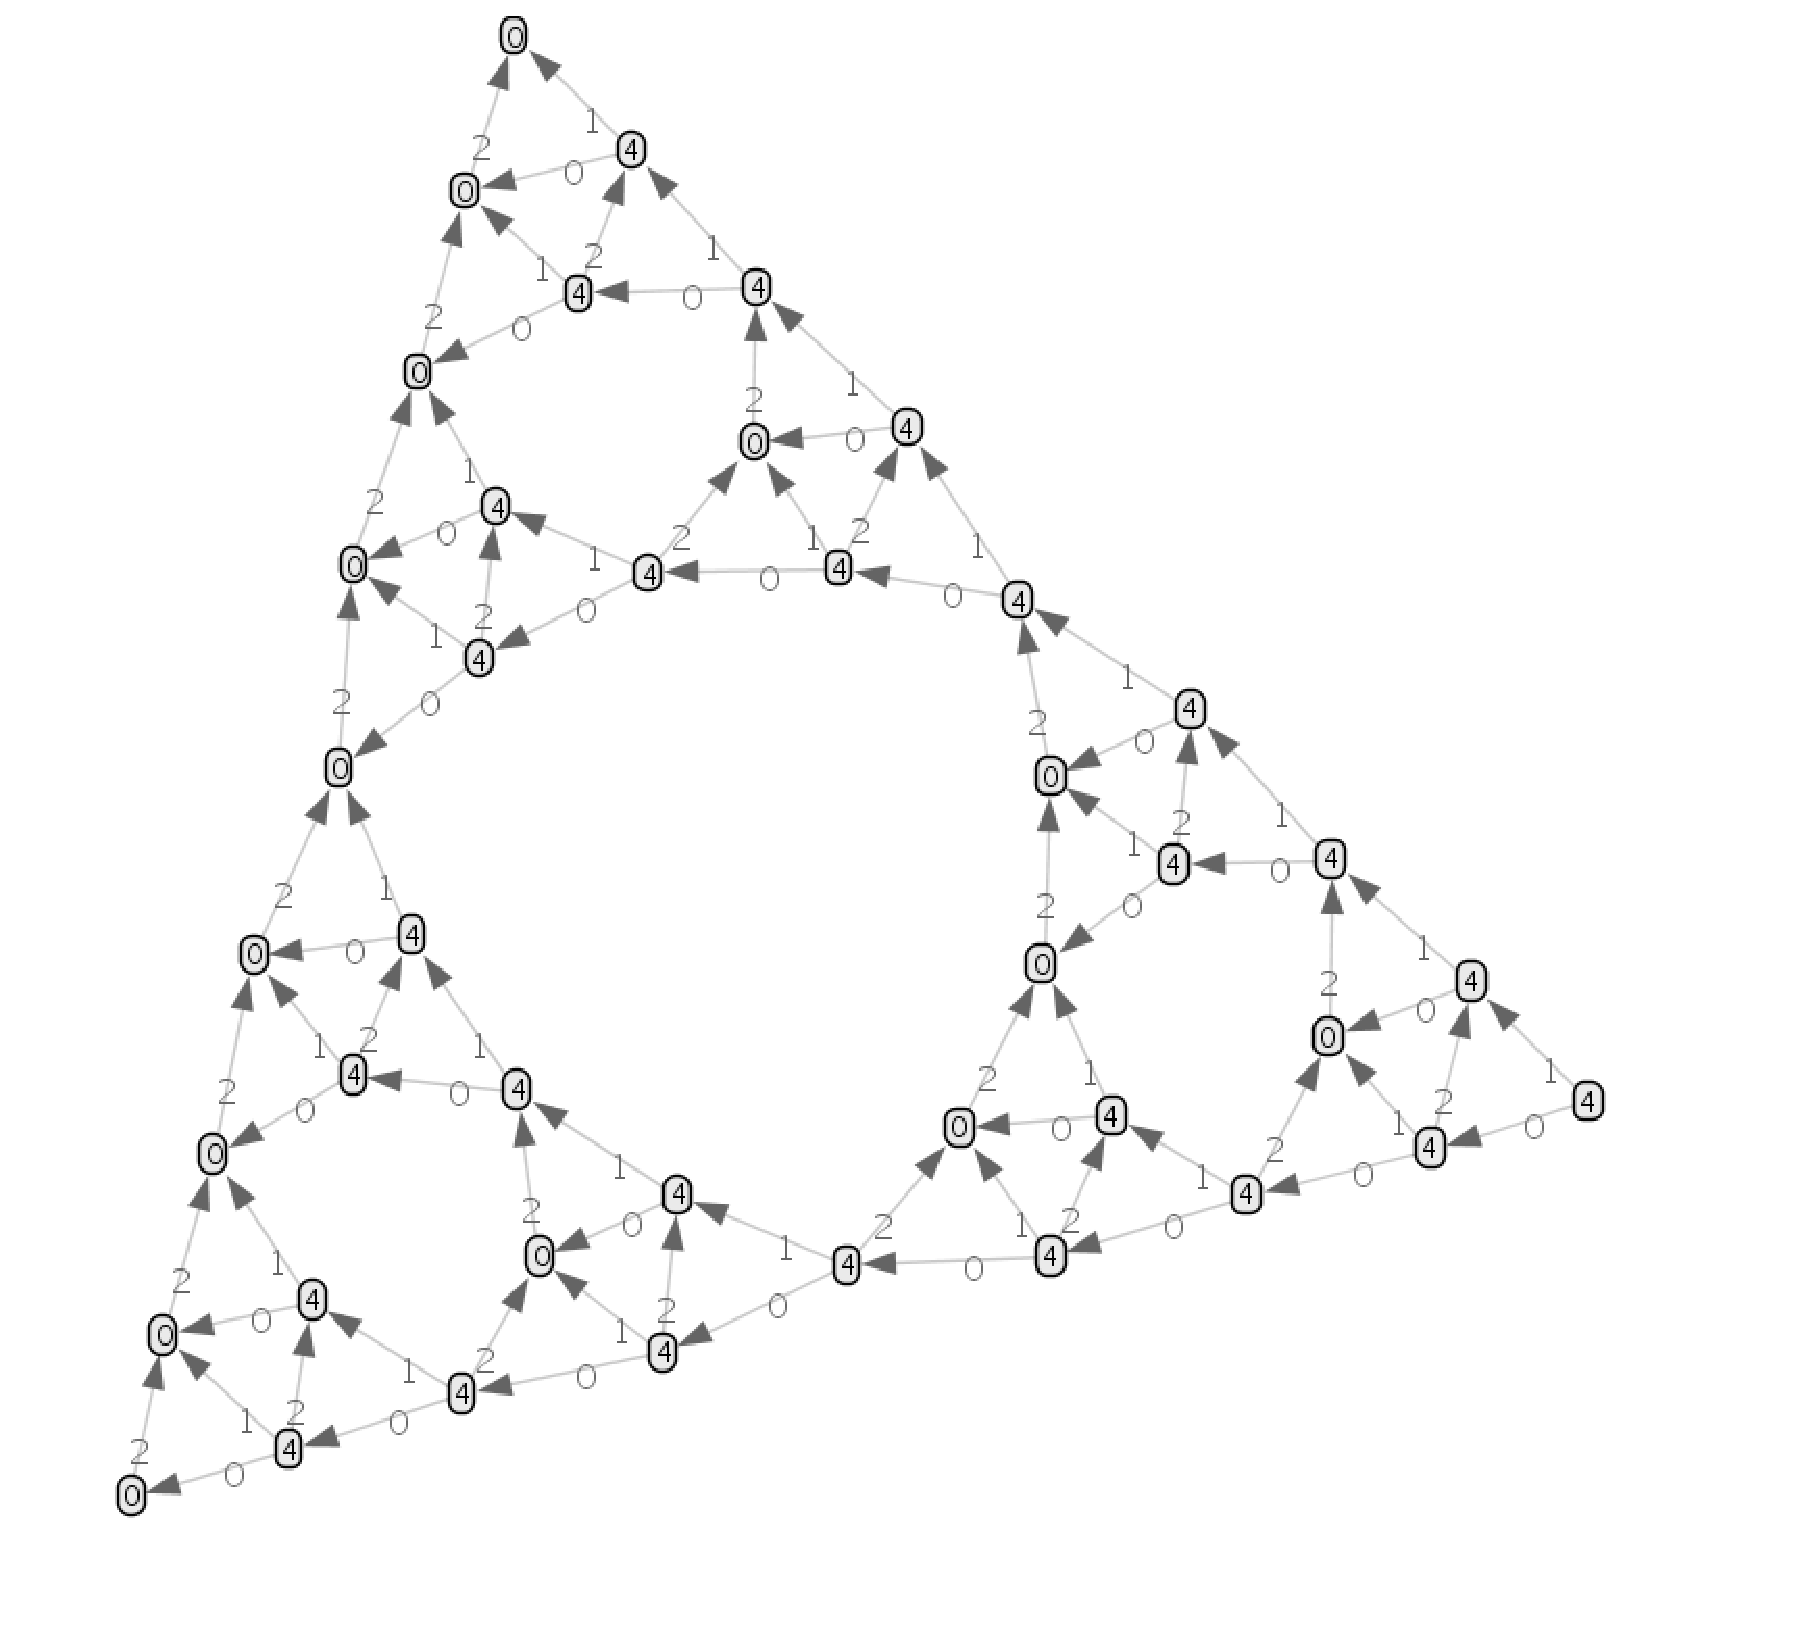
\includegraphics[scale=.35,angle=-15]{sierpinski-3.eps}
 \end{center}
\vspace*{-2.5cm}
\caption{A Sierpinski triangle (third generation)\label{fig:sierpinski}}
\end{figure}

The program in Figure \ref{fig:sierpinski-prog} expects as input a graph consisting of a single node labelled with the generation number of the Sierpinski triangle to be produced. The rule schema \texttt{init} creates the Sierpinski triangle of generation 0 and turns the input node into a unique ``control node'' with the tagged label $x\_0$ in order to hold the required generation number $x$ together with the current generation number.

After initialisation, the nested loop $\mathtt{(inc;\, expand!)!}$ is executed. In each iteration of the outer loop, \texttt{inc} increases the current generation number if it is smaller than the required number. The latter is checked by the condition \texttt{where} $\mathtt{x > y}$. If the test is successful, the inner loop \texttt{expand!} performs a Sierpinski step on each triangle whose top node is labelled with the current generation number: the triangle is replaced by four triangles such that the top nodes of the three outer triangles are labelled with the next higher generation number. The test $\mathtt{x > y}$ fails when the required generation number has been reached. In this case the application of \texttt{inc} fails, causing the outer loop to terminate and return the current graph which is the Sierpinski triangle of the requested generation.

\begin{figure}[htb]
\label{fig:sierpinski-prog}
 \begin{center}
  \input{Programs/sierpinski.prog}
 \end{center}
\caption{The program \texttt{sierpinski}}
\end{figure}

\end{example}


Figure \ref{fig:program_syntax} shows the abstract syntax of GP programs.\footnote{Where necessary we use parentheses to disambiguate programs.} A program consists of a number of declarations of conditional rule schemata and macros, and exactly one declaration of a main command sequence. 
\begin{figure}[tb]
\renewcommand{\arraystretch}{1.2}
\begin{center}
\begin{tabular}{lcl}
Prog & ::= & Decl \{Decl\} \\
Decl & ::= & RuleDecl $\mid$ MacroDecl $\mid$ MainDecl \\
MacroDecl & ::= & MacroId '=' ComSeq \\
MainDecl & ::= & \texttt{main} '=' ComSeq \\
ComSeq & ::= & Com \{';' Com\} \\
Com & ::= & RuleSetCall $\mid$ MacroCall \\
&& $\mid$ \texttt{if} ComSeq \texttt{then} ComSeq [\texttt{else} ComSeq] \\
&& $\mid$ ComSeq '!' \\
&& $\mid$ \texttt{skip} $\mid$ \texttt{fail} \\
RuleSetCall & ::= & RuleId $\mid$ '\{' [RuleId \{',' RuleId\}] '\}' \\
MacroCall & ::= & MacroId 
\end{tabular}
\end{center}
\caption{Abstract syntax of GP}\label{fig:program_syntax}
\end{figure}
The rule-schema identifiers (category RuleId) occurring in a call of category RuleSetCall refer to declarations of conditional rule schemata in category RuleDecl (see Section \ref{sec:rule_schemata}). Semantically, each rule-schema identifier $r$ stands for the set  $\I(r)$ of conditional rules induced by that identifier. A call of the form $\{r_1,\dots,r_n\}$ stands for the union $\bigcup_{i=1}^n\I(r_i)$.

Macros are a simple means to structure programs and thereby to make them more readable. Every program can be transformed into an equivalent macro-free program by replacing macro calls with their associated command sequences (recursive macros are not allowed). In the next section we use the terms ``program'' and ``command sequence'' synonymously, assuming that all macro calls have been replaced. 

The commands \texttt{skip} and \texttt{fail} can be expressed through the other commands (see next section), hence the core of GP includes only the call of a set of conditional rule schemata (RuleSetCall), sequential composition (';'), the if-then-else statement and as-long-as-possible iteration ('!'). 
